% include the figures path relative to the master file
\graphicspath{ {./content/intro/figures/} }

\section{Introduction}
\label{sec:intro}  % \label{} allows reference to this section

Eye diseases such as \gls{dr} and \gls{dme} are the most common causes of irreversible vision loss in individuals with diabetes.
Just in United States alone, health care and associated costs related to eye diseases are estimated at almost $\$$500 M~\cite{Sharma2005} with prevalent cases of \gls{dr} expected to grow exponentially affecting over 300 M people worldwide by 2025~\cite{wild2004global}.
Early detection and treatment of DR and \gls{dme} play a major role to prevent adverse effects such as blindness.
\gls{dme} is characterized as an increase in retinal thickness within one disk diameter of the fovea center with or without hard exudates and sometimes associated with cysts~\cite{ETDRSG1985}.
\gls{sdoct}~\cite{Chen2005} which images the depth of the retina with a high resolution and fast image acquisition is an adequate tool, compared to fundus images for \gls{dme} identification~\cite{abramoff2010retinal,trucco2013validating,giancardo2011textureless}.
As an example, Figure.\,\ref{fig:fig1} shows one normal B-scan and one abnormal B-scans and clearly illustrate the fact that lesions such as cysts can easily be spotted via \gls{oct} imaging.
Automated diagnosis on \gls{oct} imaging is rather new and most of the pioneer works on \gls{oct} image analysis have focused on the problem of retinal layers segmentation, which is a necessary step for retinal thickness measurements~\cite{chiu2010automatic,garvin2009automated,garvin2008intraretinal} and has also recently proven to be quite efficient for cysts segmentation~\cite{oguz2016optimal}. 
However, very few works, up to our knowledge, have addressed the specific problem of \gls{dme} and its associated features detection from \gls{oct} images. 
In this paper we propose a solution for automated detection of \gls{dme} on \gls{oct} volumes.

\begin{figure}
\centering
        \subfigure[\gls{dme}-case]{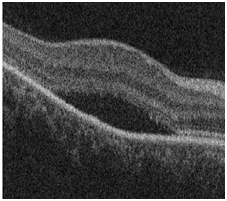
\includegraphics[width = 0.2\textwidth, height = 0.15\textheight]{dme_case}}\
        \subfigure[normal-case]{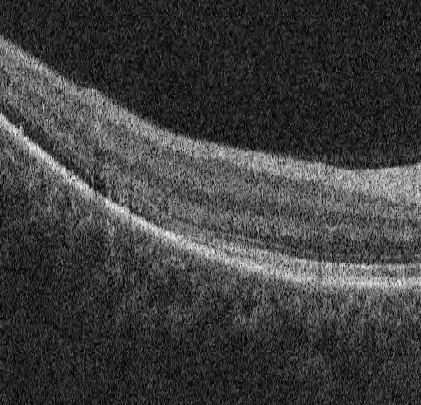
\includegraphics[width = 0.2\textwidth, height = 0.15\textheight]{normal_case2}}
\caption{\gls{dme} and normal case of \gls{oct} B-scans.}
\label{fig:fig1}
\end{figure}

Following this introduction, the rest of the paper is organized as follows, part~\ref{sec:rw} will present some related works, part~\ref{sec:data} is related to the data collection, part~\ref{sec:method} and part~\ref{sec:res} are respectively dedicated to our methodology and the obtained results.
The paper ends with a short discussion and some conclusion in part~\ref{sec:dis-con} .



% Some stuff that emac's colegues use
%%% Local Variables:
%%% mode: late
%%% TeX-master: "../../main.tex"
%%% End: \section{introduction}

